\documentclass[compress, 8pt]{beamer}
% \documentclass[handout, 8pt]{beamer}
\usepackage[utf8]{inputenc}

% Notes to self: \nts[color option]{text that is a note}
\newif\ifshowcomments
% \showcommentstrue % uncomment to show
\input{preambleB}
\usepackage[normalem]{ulem}

%%%%%%%%%%%%%%%%%%%%%%%%%%%%%%%%%%%%%%%%%%%%%%%%%%%%%%%%%%%%%%%%%%%%%%%%%%%%%%
% Paths to figures
\usepackage{subcaption}

% Avoid a warning on mac; can introduce a warning (and maybe a break) on windows
% \usepackage{etex}
% Avoid a warning
\let\Tiny=\tiny

%Information to be included in the title page:
\title{Propensity Score Matching}
\subtitle{ECON726}
\author[]{Tara Sullivan}
\institute{
Tara Sullivan \\
\textit{tara.sullivan55@login.cuny.edu}
}
\date{
\today
\nts{\\
\medskip
Notes/comments are in gray and will be excluded from the presentation.
}
}

% plot graphs with pgfplots
\usepackage{pgfplots}
\pgfplotsset{compat=newest}
\usepgfplotslibrary{groupplots}
\usepgfplotslibrary{dateplot}
\pgfplotsset{compat=newest,
    every axis/.style={
        axis y line*=left,
        axis x line*=bottom,
        % allows for multi-line legend entries
        legend style={cells={align=left}},
        % allows for multi-line titles
        title style={align=center},
    },
}

% For animations using underbrace 
% Source: https://tex.stackexchange.com/a/565866
\usepackage{xparse, letltxmacro}
\LetLtxMacro{\oldunderbrace}{\underbrace}
\DeclareDocumentCommand{\underbrace}{d<> m e{_}}{%
  \IfValueTF{#1}{% IF <overlay-specification> given
    % using global onlside flag, cf. p82 beamer manual v3.59
    \oldunderbrace{#2\onslide<#1>}_{#3}\onslide%
  }{% ELSE
    \oldunderbrace{#2}_{#3}
  }%
}%

\usetikzlibrary{decorations.pathreplacing,calligraphy}

%%%%%%%%%%%%%%%%%%%%%%%%%%%%%%%%%%%%%%%%%%%%%%%%%%%%%%%%%%%%%%%%%%%%%%%%%%%%%%%%
\begin{document}    
%\beamertemplatenavigationsymbolsempty


%%%%%%%%%%%%%%%%%%%%%%%%%%%%%%%%%%%%%%%%%%%%%%%%%%%%%%%%%%%%%%%%%%%%%%%%%%%%%%%%
\begin{frame}
\titlepage
% \tikzset{external/figure name={intro_}}
\end{frame}

%%%%%%%%%%%%%%%%%%%%%%%%%%%%%%%%%%%%%%%%%%%%%%%%%%%%%%%%%%%%%%%%%%%%%%%%%%%%%%%%
\begin{frame}{Housekeeping}

Today:
\begin{itemize}
    \item Discuss your project plan
    \item Propensity score matching
    \item Jupyter notebook: \href{https://github.com/tara-sullivan/econ726-notebooks/blob/main/notebooks/06-propensity.ipynb}{link}
\end{itemize}

\vspace{3ex}
\textbf{Homework}
\begin{itemize}
    \item Read MHE 5.1. and 5.2. (Fixed effects and differences-in-differences)
    \begin{itemize}
        \item We will focus on diff-in-diff next class, but many of your papers use fixed effects
    \end{itemize}
    \item Submit your project plan. \textbf{This is 15\% of your final grade}
    \item By next week, you need to have:
    \begin{itemize}
        \item Read your paper
        \item Verified you can access and run your replication code
        \item Submitted your project plan
        % \item There is a language to papers. You're doing your best to understand it, even if you aren't fluent
    \end{itemize}
\end{itemize}

\vspace{3ex}
\textbf{No class or office hours next week!}


\end{frame}

\begin{frame}{}

\alert{\emph{If you personally need adjustments to these deadlines let me know in advance}}

\textbf{Paper selection}: Due \textbf{\sout{September 16} September 22} [5\% of final grade]
\begin{itemize}
\item Done! 
\end{itemize}

\textbf{Project plan}: Due \textbf{October 14} [15\% of final grade] 
\begin{itemize}
\item Summarize the public policy or business context of the paper. 
Write down the specific question the paper is evaluating.
Discuss the data your are using (both your replication data, and data for your extension)
Discuss the extensions you are considering, and, if necessary, where you will be getting that data. 
\end{itemize} 

\textbf{Replication results}: \alert{Due \textbf{\sout{November 4} November 3}}: [10\% of final grade]
\begin{itemize}
\item You should submit some of your main replication results. The final results should be formatted as tables and charts in a word document or PDF, submitted on Brightspace. Your code and data should accessible on GitHub.
\end{itemize}

\textbf{Presentation}: Due \textbf{December 2} \& \textbf{December 9} [10\% of final grade]
\begin{itemize}
\item Prepare a 5-10 minute presentation on your paper. Focus on the research question, main result, and one extension. 
\end{itemize}

\textbf{Final Paper}: Due \textbf{December 16} [35\% of final grade]
\begin{itemize}
\item Your paper should contain 5-8 pages of text, and 5-8 pages of figures (double spaced, 12 point font).
You are expected to use python, and must provide the code and data to replicate your findings. 
Your final project should be submitted on Brightspace, and your code and data should be uploaded to github (note: if your data is too large to upload to github, let me know). 
\end{itemize}

\end{frame}

%%%%%%%%%%%%%%%%%%%%%%%%%%%%%%%%%%%%%%%%%%%%%%%%%%%%%%%%%%%%%%%%%%%%%%%%%%%%%%%%
\begin{frame}{Paper ideas}

Note: you might need to google for these data and code, but they are readily available on the internet. 
\begin{itemize}

    \item Matching estimators paper: Angrist (1998, tables II and V;
\href{https://www.jstor.org/stable/2998558}{link}; \href{https://economics.mit.edu/people/faculty/josh-angrist/angrist-data-archive}{data})

    \item Propensity Score Estimator: Deheija and Wahba (1999; \href{https://www.jstor.org/stable/pdf/2669919.pdf}{link}; \href{https://users.nber.org/~rdehejia/nswdata2.html}{data})

    \item Synthetic Control
    \begin{itemize}
        \item German reunification: Abadie, Diamond and Hainmuller (2015; \href{https://onlinelibrary.wiley.com/doi/abs/10.1111/ajps.12116}{link})
        \item Cost of conflict in Basque Country: Abadie and Gardeazabal (2003; \href{https://www.aeaweb.org/articles?id=10.1257/000282803321455188}{link})
        \item Smoking legislation in California: Abadie, Diamond, and Hainmuller (2010; \href{https://www.tandfonline.com/doi/abs/10.1198/jasa.2009.ap08746}{link})
    \end{itemize}
\end{itemize}

\end{frame}


%%%%%%%%%%%%%%%%%%%%%%%%%%%%%%%%%%%%%%%%%%%%%%%%%%%%%%%%%%%%%%%%%%%%%%%%%%%%%%%
\miniframesoff
\begin{frame}{Outline}
    \tableofcontents
\end{frame}
\miniframeson



%%%%%%%%%%%%%%%%%%%%%%%%%%%%%%%%%%%%%%%%%%%%%%%%%%%%%%%%%%%%%%%%%%%%%%%%%%%%%%%%
\section[Propensity Score]{Control for covariates using the Propensity Score}
\miniframesoff
\begin{frame}
    \tableofcontents[currentsection]
\end{frame}
\miniframeson
%%%%%%%%%%%%%%%%%%%%%%%%%%%%%%%%%%%%%%%%%%%%%%%%%%%%%%%%%%%%%%%%%%%%%%%%%%%%%%%%




%%%%%%%%%%%%%%%%%%%%%%%%%%%%%%%%%%%%%%%%%%%%%%%%%%%%%%%%%%%%%%%%%%%%%%%%%%%%%%%%
\begin{frame}{Review: matching}

Variables:
\begin{itemize}
    \item $Y_i$: Outcome variable
    \item $D_i$: Binary treatment dummy variable
    \item $X_i$: Covariates
\end{itemize}
Under conditional independence assumption (CIA) $\{Y_{0i}, Y_{1i}\} \perp D_i \vert X_i$, we can construct causal matching estimators:
\begin{align*}
    \delta_{ToT} &= \EE [Y_{1i} - Y_{0i} \vert D_i = 1] \\
    &= \sum_x \delta_x \PP(X_i = x \vert D_i = 1) \\
    \delta_{ATE} &= \EE [Y_{1i} - Y_{0i}] \\
    &= \sum_x \delta x \PP (X_i = x)
\end{align*}
where:
\begin{equation*}
    \delta_X = \EE [Y_i \vert X_i, D_i = 1] - \EE [Y_i \vert X_i, D_i = 0]
\end{equation*}
Note: matching and regression are both weighted averages of covariate specific differences

\end{frame}

% %%%%%%%%%%%%%%%%%%%%%%%%%%%%%%%%%%%%%%%%%%%%%%%%%%%%%%%%%%%%%%%%%%%%%%%%%%%%%%%%
% \begin{frame}{}

% Intutively matching makes sense as an estimator
% \begin{itemize}

%     \item Matching estimators paper: Angrist (1998, tables II and V):
% \href{https://www.jstor.org/stable/2998558}{link}; \href{https://economics.mit.edu/people/faculty/josh-angrist/angrist-data-archive}{data}
% \end{itemize}


% % \vspace{3ex}
% % One problem: Curse of dimensionality

% \end{frame}

%%%%%%%%%%%%%%%%%%%%%%%%%%%%%%%%%%%%%%%%%%%%%%%%%%%%%%%%%%%%%%%%%%%%%%%%%%%%%%%%
\begin{frame}{Motivating example}


``Growth mindset'' example (heavily borrows from: \href{https://matheusfacure.github.io/python-causality-handbook/11-Propensity-Score.html}{link})
\begin{itemize}
    \item If you think your intelligence is fixed, there is no incentive to study; academic outcomes are worse
    \item If you have a ``growth mindset,'' there are returns to intelligence; your academic outcomes are better
\end{itemize}

The National Study of Learning Mindsets
\begin{itemize}
    \item Evaluate the impact of a nudge-like intervention designed to instill students with a growth mindset on student achievement
\item Students randomly given the opportunity to participate in ``growth mindset'' seminar in high school; academic outcomes in college were then recorded
\item Problem: students with the highest expectation of success were more likely to receive the treatment
\begin{itemize}
    \item Opportunity to participate in the seminar was random
    \item Those who moved forward with the opportunity may have been more ambitious than those who did not
\end{itemize}
\end{itemize}

Athey and Wagner (2016) generate simulated data: \href{https://arxiv.org/pdf/1902.07409}{link}

\end{frame}

%%%%%%%%%%%%%%%%%%%%%%%%%%%%%%%%%%%%%%%%%%%%%%%%%%%%%%%%%%%%%%%%%%%%%%%%%%%%%%%%
\begin{frame}{Motivating example (cont)}

Variables:
\begin{itemize}
    \item $Y_i$: Outcome variable (achievement score in college)
    \item $D_i$: Binary treatment dummy variable (participating in ``growth mindset'') seminar
    \item $X_i$: Covariates (individual and school demographics; family characteristics; survey about expectations of future success)
\end{itemize}

\begin{figure}
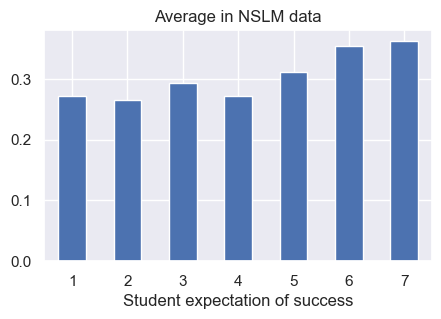
\includegraphics[scale=0.5]{img/fig-nslm-1.png}
\end{figure}
More ambitious students may be more willing to go to the seminar, leading to selection bias. How can we correct for that?

\end{frame}


%%%%%%%%%%%%%%%%%%%%%%%%%%%%%%%%%%%%%%%%%%%%%%%%%%%%%%%%%%%%%%%%%%%%%%%%%%%%%%%%
\begin{frame}[t]{Propensity Score Theorem}

Define the propensity score (or balancing score) to be:
\begin{align*}
{\color{cyan}p(X_i)} =& \mathbf{E} [D_i \vert X_i] \\
=& \sum_{d=0}^1 d \cdot \mathbf{P} (D_i = d \vert X_i) \\
=& 0 \cdot \mathbf{P} (D_i = 0 \vert X_i) + 1 \cdot \mathbf{P} (D_i = 1 \vert X_i) \\
=& {\color{Green}\mathbf{P} (D_i = 1 \vert X_i)}
\end{align*}
\textbf{Note:} the {\color{cyan}propensity score} equals the {\color{Green}probability of treatment} for binary treatments

\vspace{3ex}
Suppose the CIA holds such that $\{Y_{0i}, Y_{1i}\} \perp D_i \vert X_i$. Then $\{Y_{0i}, Y_{1i} \} \perp D_i \vert p(X_i)$

\vspace{3ex}\textbf{What does this mean?}
\begin{itemize}
    \item You don't need to directly control for confounders $X$ to achieve CIA
    \item Instead, it is sufficient to control for a single variable, $p(X_i)$
\end{itemize}


\end{frame}

%%%%%%%%%%%%%%%%%%%%%%%%%%%%%%%%%%%%%%%%%%%%%%%%%%%%%%%%%%%%%%%%%%%%%%%%%%%%%%%%
\begin{frame}[t]{}

{\color{DarkGray}\textbf{Propensity Score Theorem:} Given propensity score:
\begin{equation*}
    p(X_i) = \EE [D_i \vert X_i] = \PP (D_i = 1 \vert X_i)
\end{equation*}
Suppose the CIA holds such that $\{Y_{0i}, Y_{1i}\} \perp D_i \vert X_i$. Then $\{Y_{0i}, Y_{1i} \} \perp D_i \vert p(X_i)$
}

\vspace{3ex}
\textbf{Proof:}

First, instead of writing $\{Y_{0i}, Y_{1i}\}$, we'll write $Y_{ji}$, where $j \in {0, 1}$.

\vspace{2ex}
Next, note that the conditional expectation of the treatment variable equals the conditional probability of treatment (because the treatment is binary):
\begin{align*}
    \EE [D_i \vert Y_{ji}, p(X_i)] =& \sum_{d = 0}^1 d \PP (D_i = d \vert Y_{ji}, p(X_i)) \\
    =& 0 \cdot \PP (D_i = 0 \vert Y_{ji}, p(X_i))
    + 1 \cdot \PP (D_i = 1 \vert Y_{ji}, p(X_i)) \\
    =& \PP (D_i = 1 \vert Y_{ji}, p(X_i))
\end{align*}
\end{frame}



%%%%%%%%%%%%%%%%%%%%%%%%%%%%%%%%%%%%%%%%%%%%%%%%%%%%%%%%%%%%%%%%%%%%%%%%%%%%%%%%
\begin{frame}[t]{}

{\color{DarkGray}\textbf{Propensity Score Theorem:} Given propensity score:
\begin{equation*}
    p(X_i) = \EE [D_i \vert X_i] = \PP (D_i = 1 \vert X_i)
\end{equation*}
Suppose the CIA holds such that $\{Y_{0i}, Y_{1i}\} \perp D_i \vert X_i$. Then $\{Y_{0i}, Y_{1i} \} \perp D_i \vert p(X_i)$
}

\vspace{3ex}
\textbf{Proof:}

We want to show that:
\begin{equation*}
    {\color<2>{cyan}\EE [D_i \vert X_i, p(X_i)]}
    = 
    {\color<3>{Green}\EE [D_i \vert p(X_i)]}
\end{equation*}
\onslide<2->{
First consider the left hand side:
\begin{align*}
    {\color<2,5>{cyan}\EE [D_i \vert X_i, p(X_i)]} 
    &= \EE [D_i \vert X_i] 
    {\color<5,7>{HunterPurple}= p(X_i)}
\end{align*}
In words: $p(X_i)$ is a function of $X_i$, so conditioning on $X_i$ and $p(X_i)$ does not give any more information than conditioning on $X_i$ alone.
}

\vspace{2ex}
\onslide<3->{
    Next consider the right hand side:
    \begin{align*}
        {\color<3>{Green}\EE [D_i \vert p(X_i)] }
        % {\EE \Big[ } 
        % {\color<4>{MainBlue}\EE [}D_i \vert {\color<4>{MainBlue}X_i}, p(X_i) {\color<4>{MainBlue}]} 
        % {\Big\vert p(X_i) \Big]}
        \onslide<4->{
        &=
        {\EE \Big[ } 
        {\color<5>{cyan}
            \EE [D_i \vert {\color<4>{MainBlue}X_i}, p(X_i)]
        }
        {\Big\vert p(X_i) \Big]}
        &\because{\text{Law of iterated expectations}} \\
        }
        \onslide<5->{
        =& {\EE \Big[ } 
        {\color<5>{HunterPurple} p(X_i)}
        {\Big\vert p(X_i) \Big]}
        } \\
        \onslide<6->{
        =& {\color<7>{HunterPurple} p(X_i)}
        }
    \end{align*}
}
\onslide<7->{
    Because
    ${\color<7>{HunterPurple} p(X_i)} {\color<7>{HunterPurple}= p(X_i)}$, the statement is true.
}

\end{frame}

%%%%%%%%%%%%%%%%%%%%%%%%%%%%%%%%%%%%%%%%%%%%%%%%%%%%%%%%%%%%%%%%%%%%%%%%%%%%%%%%
\begin{frame}{}

\begin{figure}
\begin{tikzpicture}[
    node distance=1.25cm,
    every node/.style={
        draw, circle, minimum size=.85cm, align=center, inner sep=0pt
    }]

   % Nodes
  \node (X) {X};
  \node[right=of X] (pX) {$p(X)$};
  \node[right=of pX] (D) {D};
  \node[right=of D] (Y) {$Y$};

  % Arrows
  \draw[->] (X) -- (pX);
  \draw[->] (pX) -- (D);
  \draw[->] (D) -- (Y);

  % Curved arrow from X to Y
  \draw[->, bend left=40] (X) to (Y);

\end{tikzpicture}
\end{figure}
\begin{itemize}
    \item If I know what $p(X)$ is, then $X$ alone doesn't tell me anything else about what the probability of treatment is
    \item Controlling for $p(X)$ acts the same way as controlling for $X$ directly
\end{itemize}

\end{frame}

%%%%%%%%%%%%%%%%%%%%%%%%%%%%%%%%%%%%%%%%%%%%%%%%%%%%%%%%%%%%%%%%%%%%%%%%%%%%%%%%
\section[Treatment effects]{Propensity scores and treatment effects}
\miniframesoff
\begin{frame}
    \tableofcontents[currentsection]
\end{frame}
\miniframeson
%%%%%%%%%%%%%%%%%%%%%%%%%%%%%%%%%%%%%%%%%%%%%%%%%%%%%%%%%%%%%%%%%%%%%%%%%%%%%%%%

%%%%%%%%%%%%%%%%%%%%%%%%%%%%%%%%%%%%%%%%%%%%%%%%%%%%%%%%%%%%%%%%%%%%%%%%%%%%%%%%
\begin{frame}{Propensity scores and treatment effects}

How are propensity scores used in practice?
\begin{itemize}
    \item First, estimate the propensity score
    \begin{itemize}
        \item Use a parametric model, like a logit or probit model
    \end{itemize}
    \item Next generate the effect of treatment
    \begin{itemize}
        \item Match on estimated score (direct propensity score matching)
        \item OR use weighting scheme described next
    \end{itemize}
\end{itemize}

\end{frame}

%%%%%%%%%%%%%%%%%%%%%%%%%%%%%%%%%%%%%%%%%%%%%%%%%%%%%%%%%%%%%%%%%%%%%%%%%%%%%%%%
\begin{frame}{Direct propensity score matching}

Given a propensity score, $p(X_i)$, and the CIA $\{Y_{0i}, Y_{1i}\} \perp D_i \vert X_i$:
\begin{align*}
    \delta_{ToT} =& \EE [Y_{1i} - Y_{0i} \vert D_i = 1] \\
    =& \EE \left[
        \EE [Y_i \vert p(X_i), D_i = 1]
        - \EE [Y_i\vert p(X_i), D_i = 0]
    \right]
\end{align*}
Just like we did for matching, you can
\begin{itemize}
    \item Stratify the sample in to values of $p(X_i)$
    \item Find treatment effects conditional on similar $p(X_i)$
    \item Weigh these treatment effects by the distribution of $p(X_i)$ conditional on treatment
\end{itemize}

\end{frame}

%%%%%%%%%%%%%%%%%%%%%%%%%%%%%%%%%%%%%%%%%%%%%%%%%%%%%%%%%%%%%%%%%%%%%%%%%%%%%%%%
\begin{frame}{Propensity score weights}

Alternative: estimate treatment effects using propensity score weights. Final equation:
\begin{equation*}
    \mathbf{E} [Y_{1i} - Y_{0i}]
    = \mathbf{E} \left[ \frac{Y_i \left[ D_i - p(X_i) \right]}{p(X_i) (1 - p(X_i))} \right] 
\end{equation*}
We'll go through the math. Motivation for this method:
\begin{itemize}
    \item Avoids the matching step
    \item The concept of inverse probability weighting is important in more advanced topics
\end{itemize}
To prove this, we'll have to prove a few interim steps

\end{frame}

%%%%%%%%%%%%%%%%%%%%%%%%%%%%%%%%%%%%%%%%%%%%%%%%%%%%%%%%%%%%%%%%%%%%%%%%%%%%%%%%
\begin{frame}[t]{}

{\color{DarkGray}
\textbf{Fact \#1:}
\begin{equation*}
    \EE \left[ \frac{Y_i D_i}{p(X_i)} \right] = \EE [Y_{1i}]
\end{equation*}
}

\vspace{2ex}
\onslide<2->{
\textbf{Proof:}
First note that \alert<5>{$D_i = D_i^2$} for $D_i = 0$ and $D_i = 1$.    

\onslide<3->{
\vspace{1ex}
Next, recall \alert<3>{$Y_i = Y_{0i} + (Y_{1i} - Y_{0i}) D_i$}:
\begin{align*}
Y_i D_i =& \alert<3>{(Y_{0i} + (Y_{1i} - Y_{0i}) D_i)} D_i \\
\onslide<4->{=& Y_{0i} D_i + (Y_{1i} - Y_{0i}) \alert<5>{D_i^2} \\}
\onslide<5->{=& Y_{0i} D_i + (Y_{1i} - Y_{0i}) \alert<5>{D_i} \\
=& Y_{1i} D_i}
\end{align*}

\onslide<6->{
Using the above equality, the conditional independence assumption, and the definition of the propensity score:
\begin{align*}
\mathbf{E} [ Y_i D_i \vert X_i ]
=& \mathbf{E} [ Y_{1i} D_i \vert X_i ]  &&\because Y_i D_i = Y_{1i} D_i \\
\onslide<7->{
=& \mathbf{E} [Y_{1i} \vert X_i ] \cdot \mathbf{E} [D_i \vert X_i ] &&\because \left. Y_{1i} \perp D_i \right\vert X_i\\}
\onslide<8->{=& \mathbf{E} [Y_{1i} \vert X_i ] p(X_i) &&\because p(X_i) = \mathbf{E} [D_i \vert X_i ]}
\end{align*}

} % \onslide<6->
} % \onslide<3->
} % \onslide<2->

\end{frame}

%%%%%%%%%%%%%%%%%%%%%%%%%%%%%%%%%%%%%%%%%%%%%%%%%%%%%%%%%%%%%%%%%%%%%%%%%%%%%%%%
\begin{frame}[t]{}

{\color{DarkGray}
\textbf{Fact \#1:}
\begin{equation*}
    \EE \left[ \frac{Y_i D_i}{p(X_i)} \right] = \EE [Y_{1i}]
\end{equation*}
}

\vspace{2ex}
\textbf{Proof: (cont.)}

\onslide<2->{  
\vspace{1ex}
We've seen:
\begin{equation*}
    \mathbf{E} [ Y_i D_i \vert X_i ] = \mathbf{E} [Y_{1i} \vert X_i ] p(X_i)
\end{equation*}

\vspace{1ex} Now we can estimate $\mathbf{E} \left[ \frac{Y_i D_i}{p(X_i)} \right]$:
\begin{align*}
\onslide<3->{
\mathbf{E} \left[ \frac{Y_i D_i}{p(X_i)} \right] =&
\mathbf{E} \left[ \mathbf{E} \left[ \left. \frac{Y_i D_i}{p(X_i)} \right\vert X_i \right] \right] 
&&\because \text{Law of iterated expectations} \\}
\onslide<4->{
=&  \mathbf{E} \left[ \frac{1}{p(X_i)} \mathbf{E} \left[  \left. Y_i D_i \right\vert X_i \right] \right] \\}
\onslide<5->{
=&  \mathbf{E} \left[ \frac{1}{p(X_i)} \mathbf{E} [Y_{1i} \vert X_i ] p(x) \right]
&&\because \mathbf{E} [ Y_i D_i \vert X_i ] = \mathbf{E} [Y_{1i} \vert X_i] p(X_i) \\}
\onslide<6->{
=&  \mathbf{E} \left[ \frac{p(X_i)}{p(X_i)} \mathbf{E} [Y_{1i} \vert X_i ] \right] \\
}
\onslide<7->{
=& \mathbf{E} [Y_{1i}]
&&\because \text{Law of iterated expectations}
}
\end{align*}


} % \onslide<2->
\end{frame}

%%%%%%%%%%%%%%%%%%%%%%%%%%%%%%%%%%%%%%%%%%%%%%%%%%%%%%%%%%%%%%%%%%%%%%%%%%%%%%%%
\begin{frame}[t]{}

{\color{DarkGray}
\textbf{Fact \#2:}
\begin{equation*}
    \mathbf{E} \left[ \frac{Y_i (1 - D_i)}{1 - p(X_i)} \right] = \mathbf{E} [Y_{0i}]
\end{equation*}
}

\vspace{2ex}
\textbf{Proof:}
Recall {$Y_i = Y_{0i} + (Y_{1i} - Y_{0i})$}, and note $D_i (1 - D_i) = 0$ for $D_i = 0$ and $D_i = 1$:
\begin{align*}
Y_i (1 - D_i) 
\onslide<2->{=& (Y_{0i} + (Y_{1i} - Y_{0i}) D_i) (1 - D_i) \\}
\onslide<3->{=& Y_{0i} (1 - D_i) + (Y_{1i} - Y_{0i}) D_i (1 - D_i) \\}
\onslide<4->{
=& Y_{0i} (1 - D_i) + (Y_{1i} - Y_{0i}) \cdot 0 \\}
\onslide<5->{
=& Y_{0i} (1 - D_i)}
\end{align*}

\onslide<6->{
Using the above equality, the conditional independence assumption, and the definition of the propensity score:
\begin{align*}
\mathbf{E} [ Y_i (1 - D_i) \vert X_i ]
=& \mathbf{E} \left[ \left. Y_{0i} (1 - D_i) \right\vert X_i \right] \\
\onslide<7->{
=& \mathbf{E} [ Y_{0i} \vert X_i ] \cdot \mathbf{E} [1 - D_i \vert X_i]
&&\because \left. Y_{0i} \perp D_i \right\vert X_i\\}
\onslide<8->{=& \mathbf{E} [ Y_{0i} \vert X_i ] (1 - p(X_i))}
\end{align*}


} % \onslide<6->
\end{frame}

%%%%%%%%%%%%%%%%%%%%%%%%%%%%%%%%%%%%%%%%%%%%%%%%%%%%%%%%%%%%%%%%%%%%%%%%%%%%%%%%
\begin{frame}{}

{\color{DarkGray}
\textbf{Fact \#2:}
\begin{equation*}
    \mathbf{E} \left[ \frac{Y_i (1 - D_i)}{1 - p(X_i)} \right] = \mathbf{E} [Y_{0i}]
\end{equation*}
}

\vspace{2ex}
\textbf{Proof (cont.):}

\vspace{1ex}
We've seen:
\begin{equation*}
    \alert<4>{\mathbf{E} [ Y_i (1 - D_i) \vert X_i ]
    = \mathbf{E} [ Y_{0i} \vert X_i ] (1 - p(X_i))}
\end{equation*}
Now we can estimate $\mathbf{E} \left[ \frac{Y_i (1 - D_i)}{1 - p(X_i)} \right]$:
\begin{align*}
\onslide<2->{
\mathbf{E} \left[ \frac{Y_i (1 - D_i)}{1 - p(X_i)} \right]
=& \mathbf{E} \left[ \mathbf{E} \left[ \left. \frac{Y_i (1 - D_i)}{1 - p(X_i)} \right\vert X_i \right] \right]
&&\because \text{Law of iterated expectations} \\}
\onslide<3->{
=& \mathbf{E} \left[ \frac{1}{1 - p(X_i)} 
\alert<4>{\mathbf{E} \left[ \left. Y_i (1 - D_i) \right\vert X_i \right]} \right] \\}
\onslide<4->{
=& \mathbf{E} \left[ \frac{1}{1 - p(X_i)} 
\alert<4>{\mathbf{E} [ Y_{0i} \vert X_i ] (1 - p(X_i))} \right] 
% &&\because \mathbf{E} [ Y_i (1 - D_i) \vert X_i ] = \mathbf{E} [ Y_{0i} \vert X_i ] (1 - p(X_i))
\\}
\onslide<5->{
=& \mathbf{E} \left[\mathbf{E} [ Y_{0i} \vert X_i ] \right] \\}
\onslide<6->{
=& \mathbf{E} [Y_{0i}] 
&&\because \text{Law of iterated expectations}}
\end{align*}


\end{frame}

%%%%%%%%%%%%%%%%%%%%%%%%%%%%%%%%%%%%%%%%%%%%%%%%%%%%%%%%%%%%%%%%%%%%%%%%%%%%%%%%
\begin{frame}{}

We've seen
\begin{equation*}
\EE \left[ \frac{Y_i D_i}{p(X_i)} \right] = \EE [Y_{1i}],
\quad \quad
    \mathbf{E} \left[ \frac{Y_i (1 - D_i)}{1 - p(X_i)} \right] = \mathbf{E} [Y_{0i}]
\end{equation*}
Average treatment effects can be estimated from:
\begin{align*}
\mathbf{E} [Y_{1i} - Y_{0i}]
=& \mathbf{E} 
\left[ 
    \frac{Y_i D_i}{p(X_i)}
    - \frac{Y_i (1 - D_i)}{1 - p(X_i)}
\right] \\
=& \mathbf{E} \left[ \frac{Y_i D_i (1 - p(X_i)) - Y_i (1 - D_i) p(X_i)}{p(X_i) (1 - p(X_i))} \right] \\
=& \mathbf{E} \left[ \frac{Y_i \left[ D_i (1 - p(X_i)) - (1 - D_i) p(X_i) \right]}{p(X_i) (1 - p(X_i))} \right] \\
=& \mathbf{E} \left[ \frac{Y_i \left[ D_i - D_i p(X_i) - p(X_i) +  D_i p(X_i) \right]}{p(X_i) (1 - p(X_i))} \right] \\
=& \mathbf{E} \left[ \frac{Y_i \left[ D_i - p(X_i) \right]}{p(X_i) (1 - p(X_i))} \right] \\
\end{align*}

\end{frame}

%%%%%%%%%%%%%%%%%%%%%%%%%%%%%%%%%%%%%%%%%%%%%%%%%%%%%%%%%%%%%%%%%%%%%%%%%%%%%%%%
\begin{frame}{}

Horvitz-Thompson Propensity score weighting:
\begin{equation*}
    \mathbf{E} [Y_{1i} - Y_{0i}]
    = \mathbf{E} \left[ \frac{Y_i \left[ D_i - p(X_i) \right]}{p(X_i) (1 - p(X_i))} \right]
\end{equation*}
\begin{itemize}
    \item Uses propensity score weighting to recover average treatment effects
    \item Using the propensity score rather than identification by conditioning on $X$ is a useful empirical strategy when $X$ is high-dimensional and $p(X)$ is available (or can be approximated accurately)
    \item MHE shows how this can be considered similar to the regression estimator
\end{itemize}


\end{frame}




%%%%%%%%%%%%%%%%%%%%%%%%%%%%%%%%%%%%%%%%%%%%%%%%%%%%%%%%%%%%%%%%%%%%%%%%%%%%%%
\section[Extensions]{Important extensions}
\miniframesoff
\begin{frame}
    \tableofcontents[currentsection]
\end{frame}
\miniframeson
%%%%%%%%%%%%%%%%%%%%%%%%%%%%%%%%%%%%%%%%%%%%%%%%%%%%%%%%%%%%%%%%%%%%%%%%%%%%%%

%%%%%%%%%%%%%%%%%%%%%%%%%%%%%%%%%%%%%%%%%%%%%%%%%%%%%%%%%%%%%%%%%%%%%%%%%%%%%%
\begin{frame}{Inverse Probability of Treatment Weighting}
We've seen:
\begin{equation*}
{\color<6>{DarkGray}\EE \left[ \frac{{\color<2>{cyan}Y_i D_i}}{{\color<3-4>{cyan} p(X_i)}} \right] = \EE [Y_{1i}]},
\quad \quad
{\color<2-5>{DarkGray}\mathbf{E} \left[ \frac{Y_i (1 - D_i)}{1 - p(X_i)} \right] = \mathbf{E} [Y_{0i}]}
\end{equation*}
Consider the first element:
\begin{itemize}
    \onslide<2->{\item {\color<2>{cyan} $Y_i D_i$}: Isolates $Y_i$ that are treated}
    \onslide<3->{\item {\color<3-4>{cyan} $p(X_i)$}: Inverse probability of being treated
    \onslide<4->{
    \begin{itemize}
        \item Probabilities are between 0 and 1
        \item Low probability events $\implies$ inverse probability high
        \begin{align*}
            p(X) = 0.1 = \frac{1}{10} \implies& \frac{1}{p(X)} = \frac{1}{1/10} = 10
        \end{align*}
        \item High probability events $\implies$ inverse probability low
        \begin{align*}
p(X) = 0.8 = \frac{4}{5} \implies& \frac{1}{p(X)} = \frac{1}{4/5} = 1.25
        \end{align*} 
    \end{itemize}
    \onslide<5->{
    \item Treated observations with a low $p(X)$ probably look more like the untreated. Therefore, they receive greater weight. Vice versa for the untreated
    }
    }}
\end{itemize}
\onslide<6->{The same reasoning applies to the second element}

\vspace{3ex}
\onslide<7->{IPTW: valuable in a clinical setting to generate balanced data}

\end{frame}

%%%%%%%%%%%%%%%%%%%%%%%%%%%%%%%%%%%%%%%%%%%%%%%%%%%%%%%%%%%%%%%%%%%%%%%%%%%%%%%%
\begin{frame}{Structural model and connection to machine learning}

Note: the following is from \emph{Business Data Science} by Matt Taddy, Chapter 6

\vspace{3ex}
Consider a common structural model:
\begin{align*}
    Y &= D \gamma + X^\prime \beta + \epsilon, \quad \epsilon \vert D, X = 0 \\
    D &= X^\prime \tau + v, \quad v \vert X = 0
\end{align*}
Note:
\begin{itemize}
    \item $\epsilon \vert D, X = 0$ and $v \vert X = 0$ encode CIA
\end{itemize}
Two-step \textbf{linear treatment effects (LTE)} model
\begin{itemize}
    \item First estimate treatment $D_i$
    \item Then estimate treatment effects $\gamma$
\end{itemize}
Dimensionality starts to matter here
\begin{itemize}
    \item If $n$ (number of observations) are much greater than $p$ (number of $X$ variables), you can use regression models
    \item If you don't have $n>>p$, traditional methods break down
\end{itemize}
\end{frame}

%%%%%%%%%%%%%%%%%%%%%%%%%%%%%%%%%%%%%%%%%%%%%%%%%%%%%%%%%%%%%%%%%%%%%%%%%%%%%%%%
\begin{frame}{Estimation of LTE}
Structural model:
\begin{align*}
    Y &= D \gamma + X^\prime \beta + \epsilon, \quad \epsilon \vert D, X = 0 \\
    D &= X^\prime \tau + v, \quad v \vert X = 0
\end{align*}
Estimation procedure:
\begin{enumerate}
    \item Estimate $\EE [D \vert X] = X^\prime \tau$. Collect fitted values
    $\hat{D} = X^\prime \hat{\tau}$
    \item Estimate:
    \begin{equation*}
        \EE [Y \vert X, D] = \hat{D} \psi + D \gamma + X^\prime \beta
    \end{equation*}
\end{enumerate}
The $\psi$ is the treatment effect of $D$ on $Y$.

\end{frame}

%%%%%%%%%%%%%%%%%%%%%%%%%%%%%%%%%%%%%%%%%%%%%%%%%%%%%%%%%%%%%%%%%%%%%%%%%%%%%%%%
\begin{frame}{LTE and propensity score matching}

Structural model in propensity score models:
\begin{align*}
    Y &= D \gamma + X^\prime \beta + \epsilon, \quad \epsilon \vert D, X = 0 \\
    D &\sim \text{Bernoulli}\left( p(X) \right) \\
    p(X) &= \frac{e^{X^\prime \tau}}{1 + e^{X^\prime \tau}}
\end{align*}
\begin{itemize}
    \item $D$ is modeled from a Bernoulli distribution (i.e. coin toss) with probability $p$
    \item The probability that $D=1$ is modeled using a \textbf{logistic regression}
\end{itemize}
Once you estimate the propensity score $p(X)$, you can find treatment effects by:
\begin{enumerate}
    \item Fitting the linear regression: $\EE [Y \vert D, \hat{p} (X)] = \alpha + D \gamma + \hat{p}(X) \psi$
    \item Constructing propensity score weighting estimates: $\EE \left[ \left. \frac{Y}{\hat{p(X)}} \right\vert D \right] = \alpha + D \gamma$ 
    \item Matching 
\end{enumerate}

\end{frame}

%%%%%%%%%%%%%%%%%%%%%%%%%%%%%%%%%%%%%%%%%%%%%%%%%%%%%%%%%%%%%%%%%%%%%%%%%%%%%%%%
\begin{frame}{}

Hahn (1998) shows there is a cost to propensity score matching in terms of asymptotic efficiency
\begin{itemize}
    \item What is the advantage of, say, controlling for propensity score instead of controlling for covariates in a regression?
\end{itemize}

\vspace{2ex}
MHE : ``An essential element of  propensity score methods is the use of prior knowledge for dimension reduction. The statistical payoff is an improvement in finite sample behavior. If you're not prepared to smooth, restrict, or otherwise reduce the dimensionality of the matching problem in a manner that has real empirical consequences, the you might as well go for full covariate matching or saturated regression control.''
\begin{itemize}
    \item This is very prescient! Now, in the era of big data, dimensionality reduction is key
    \item Propensity scores have a new value in double-robust machine learning; see chapter 9 of \url{https://chapters.causalml-book.org/CausalML_chap_9.pdf}
\end{itemize}

\end{frame}

% %%%%%%%%%%%%%%%%%%%%%%%%%%%%%%%%%%%%%%%%%%%%%%%%%%%%%%%%%%%%%%%%%%%%%%%%%%%%%%%%
% \begin{frame}{}

% Doudbly robust?

% \end{frame}





%%%%%%%%%%%%%%%%%%%%%%%%%%%%%%%%%%%%%%%%%%%%%%%%%%%%%%%%%%%%%%%%%%%%%%%%%%%%%%
\section[Logit models]{Logistic regression}
\miniframesoff
\begin{frame}
    \tableofcontents[currentsection]
\end{frame}
\miniframeson
%%%%%%%%%%%%%%%%%%%%%%%%%%%%%%%%%%%%%%%%%%%%%%%%%%%%%%%%%%%%%%%%%%%%%%%%%%%%%%

%%%%%%%%%%%%%%%%%%%%%%%%%%%%%%%%%%%%%%%%%%%%%%%%%%%%%%%%%%%%%%%%%%%%%%%%%%%%%%%%
\begin{frame}{Why logistic regression}

\begin{itemize}
    \item We have to use some estimation procedure to predict propensity scores $p(X)$
    \item Logistic regression is a common method
    \item Quick review of logistic regression and generalized linear models
\end{itemize}

\end{frame}

%%%%%%%%%%%%%%%%%%%%%%%%%%%%%%%%%%%%%%%%%%%%%%%%%%%%%%%%%%%%%%%%%%%%%%%%%%%%%%%%
\begin{frame}{Linear regression}

Assume we have data $\{y_i, x_{1i}, x_{2i}, \dots, x_{ki}\} = \{y_i, \mathbf{x}_i\}$. A linear regression model takes the form:
\begin{equation*}
    y_i = \beta_0 + \beta_1 x_{1i} + \beta_2 x_{2i} + \dots + \beta_k x_{ki} + \epsilon_i = \mathbf{x}_i^T \boldsymbol{\beta} + \epsilon_i, \quad i = 1, \dots, n
\end{equation*}
We can stack these equations for all $n$ equations in the data:
\begin{equation*}
    \mathbf{y} = \mathbf{X} \boldsymbol{\beta} + \boldsymbol{\epsilon}
\end{equation*}
To estimate this model using least squares, find the coefficient matrix $\boldsymbol{\beta}$ that minimizes the sum of squared residuals:
\begin{equation*}
    \hat{\boldsymbol{\beta}} = \arg \min_{\boldsymbol{\beta}} 
    = \sum_{i = 1}^n \left( y_i - \sum_{j=1}^K x_{ji} \beta_j \right)^2
\end{equation*}
A more math-y way of saying this using norm notation:
\begin{equation*}
    \hat{\boldsymbol{\beta}} = \arg \min_{\boldsymbol{\beta}} 
    \left\vert \left\vert
    \mathbf{y} - \mathbf{X} \boldsymbol{\beta}
    \right\vert\right\vert^2
\end{equation*}
\begin{itemize}
    \item Just think about the norm notation $\vert \vert \cdot \vert \vert$ communicating size in a multidimensional space
\end{itemize}
\end{frame}

%%%%%%%%%%%%%%%%%%%%%%%%%%%%%%%%%%%%%%%%%%%%%%%%%%%%%%%%%%%%%%%%%%%%%%%%%%%%%%%%
\begin{frame}{Limitations of linear model}

We are trying to predict treatment, $D_i$
\begin{itemize}
    \item Always takes on values equal to zero or 1
    \item Do we really want a linear model?
\end{itemize}
Consider data on hours studied and passing/failing a test ($D=1$ implies a student passed)

\begin{figure}
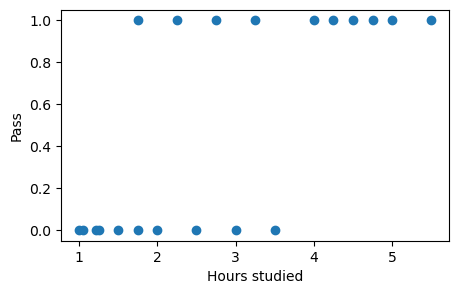
\includegraphics[scale=0.5]{img/fig-scatter.png}
\end{figure}

\end{frame}

%%%%%%%%%%%%%%%%%%%%%%%%%%%%%%%%%%%%%%%%%%%%%%%%%%%%%%%%%%%%%%%%%%%%%%%%%%%%%%%%
\begin{frame}{OLS}

We could estimate using a linear model:

\begin{figure}
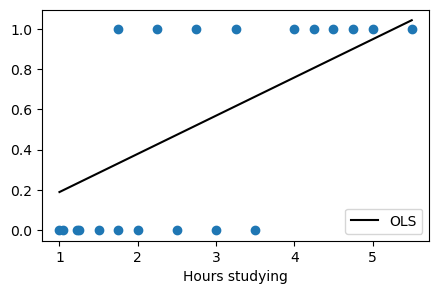
\includegraphics[scale=0.5]{img/fig-ols.png}
\end{figure}
\begin{itemize}
    \item Line isn't a great fit
\end{itemize}

\end{frame}

%%%%%%%%%%%%%%%%%%%%%%%%%%%%%%%%%%%%%%%%%%%%%%%%%%%%%%%%%%%%%%%%%%%%%%%%%%%%%%%%
\begin{frame}{Logit}

We could estimate using a linear model:

\begin{figure}
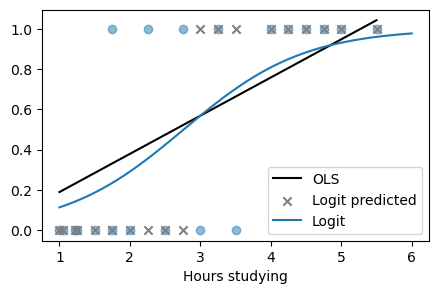
\includegraphics[scale=0.5]{img/fig-ols_logit.png}
\end{figure}
\begin{itemize}
    \item Logistic line is a better fit
    \item Less important: output is binary
\end{itemize}

\end{frame}





% %%%%%%%%%%%%%%%%%%%%%%%%%%%%%%%%%%%%%%%%%%%%%%%%%%%%%%%%%%%%%%%%%%%%%%%%%%%%%%%
% \begin{frame}{}

% \textbf{Fact #1:}
% % \begin{equation*}
% %     % \EE \left[ \frac{Y_i D_i}{p(X_i)} \right] = \EE [Y_{1i}]
% %     \mathbf{E} \left[ \frac{Y_i D_i}{p(X_i)} \right] = \mathbf{E} [Y_{1i}]
% % \end{equation*}


% \end{frame}


\end{document}
